\mySection{7.5  Drawing Inferences About $\sigma^2$}
%-------------- start slide -------------------------------%{{{ 7.47
\begin{frame}
	% {\S\: 7.5  Drawing Inferences About $\sigma^2$}
\begin{itemize}
	\item[]  For a random sample of size $n$ from $N(\mu,\sigma^2)$:
	\begin{align*}
	&S^2 =\frac{1}{n-1}\sum_{i=1}^n \left(Y_i-\overline{Y}\right)^2
	\pause \\ &\hspace{5em} \Downarrow\\
	&\frac{(n-1)S^2}{\sigma^2} = \frac{1}{\sigma^2}\sum_{i=1}^n \left(Y_i-\overline{Y}\right)^2
	\sim \text{Chi Square}(n-1)
	\end{align*}
	\item[] \pause
	\[
	\bbP\left(\chi_{\alpha/2,n-1}^2 \le \frac{(n-1)S^2}{\sigma^2}\le \chi_{1-\alpha/2,n-1}^2 \right)=1-\alpha.
	\]
\end{itemize}
\vfill
\pause
\begin{minipage}{0.45\textwidth}
	\centering
	$100(1-\alpha)\%$ C.I. for $\sigma^2$:
	\[
		\left(\frac{(n-1)s^2}{\chi^2_{1-\alpha/2,n-1}},  \frac{(n-1)s^2}{\chi^2_{\alpha/2,n-1}}\right)
	\]
\end{minipage}
\quad
\begin{minipage}{0.45\textwidth}
	\centering
	$100(1-\alpha)\%$ C.I. for $\sigma$:
	\[
		\left(\sqrt{\frac{(n-1)s^2}{\chi^2_{1-\alpha/2,n-1} }},  \sqrt{\frac{(n-1)s^2}{\chi^2_{\alpha/2,n-1} }}\right)
	\]
\end{minipage}
\end{frame}
%-------------- end slide -------------------------------%}}}
%-------------- start slide -------------------------------%{{{ 7.48
\begin{frame}
\centering
Testing $H_0:\sigma^2 = \sigma_0^2$ \\[1em] v.s.\\[1em]
(at the $\alpha$ level of significance)
\\[1em]
$\chi^2 = \frac{(n-1)s^2}{\sigma_0^2}$
\vfill

\begin{minipage}{0.32\textwidth}
\centering
$H_1:\sigma^2<\sigma_0^2$:\\[1em]
Reject $H_0$ if \\[1em]
$\chi^2 \le \chi_{\alpha,n-1}^2$
\end{minipage}
\begin{minipage}{0.32\textwidth}
\centering
$H_1:\sigma^2\ne \sigma_0^2$:\\[1em]
Reject $H_0$ if \\[1em]
$\chi^2 \le \chi_{\alpha/2,n-1}^2$ or \\[1em]
$\chi^2 \ge \chi_{1-\alpha/2,n-1}^2$
\end{minipage}
\begin{minipage}{0.32\textwidth}
\centering
$H_1:\sigma^2>\sigma_0^2$:\\[1em]
Reject $H_0$ if \\[1em]
$\chi^2 \ge \chi_{1-\alpha,n-1}^2$
\end{minipage}
\end{frame}
%-------------- end slide -------------------------------%}}}
%-------------- start slide -------------------------------%{{{ 7.49
\begin{frame}

\begin{enumerate}
\item[E.g. 1.] The width of a confidence interval for $\sigma^2$ is a function of $n$ and $S^2$:
\[
W=\frac{(n-1)S^2}{\chi^2_{\alpha/2,n-1}}-\frac{(n-1)S^2}{\chi^2_{1-\alpha/2,n-1}}
\]
Find the smallest $n$ such that the average width of a $95\%$ C.I. for $\sigma^2$ is no greater than $0.8 \sigma^2$.
\vfill
\item[Sol.] Notice that $\E[S^2]=\sigma^2$. Hence, we need to find $n$ s.t.
	\[
		(n-1)\left(\frac{1}{\chi_{0.025,n-1}^2} - \frac{1}{\chi_{0.975,n-1}^2}\right)\le 0.8.
	\]
\item[] Trial and error (numerics on R) gives $n=57$.
\end{enumerate}
\end{frame}
%-------------- end slide -------------------------------%}}}
%-------------- start slide -------------------------------%{{{ 7.50
\begin{frame}[fragile]
\begin{center}
\begin{minipage}{0.6\textwidth}
\begin{lstlisting}
> # Example 7.5.1
> n=seq(45,60,1)
> l=qchisq(0.025,n-1)
> u=qchisq(0.975,n-1)
> e=(n-1)* (1/l-1/u)
> m=cbind(n,l,u,e)
> colnames(m) = c("n",
+                 "chi(0.025,n-1)",
+                 "chi(0.975,n-1)",
+                 "error")
> m
       n chi(0.025,n-1) chi(0.975,n-1)     error
 [1,] 45       27.57457       64.20146 0.9103307
 [2,] 46       28.36615       65.41016 0.8984312
 [3,] 47       29.16005       66.61653 0.8869812
 [4,] 48       29.95620       67.82065 0.8759533
 [5,] 49       30.75451       69.02259 0.8653224
 [6,] 50       31.55492       70.22241 0.8550654
 [7,] 51       32.35736       71.42020 0.8451612
 [8,] 52       33.16179       72.61599 0.8355901
 [9,] 53       33.96813       73.80986 0.8263340
[10,] 54       34.77633       75.00186 0.8173761
[11,] 55       35.58634       76.19205 0.8087008
[12,] 56       36.39811       77.38047 0.8002937

[13,] 57       37.21159       78.56716 0.7921414
[14,] 58       38.02674       79.75219 0.7842313
[15,] 59       38.84351       80.93559 0.7765517
[16,] 60       39.66186       82.11741 0.7690918
\end{lstlisting}
\end{minipage}
	\end{center}
\end{frame}
%-------------- end slide -------------------------------%}}}
%-------------- start slide -------------------------------%{{{ 7.51
\begin{frame}
\centering
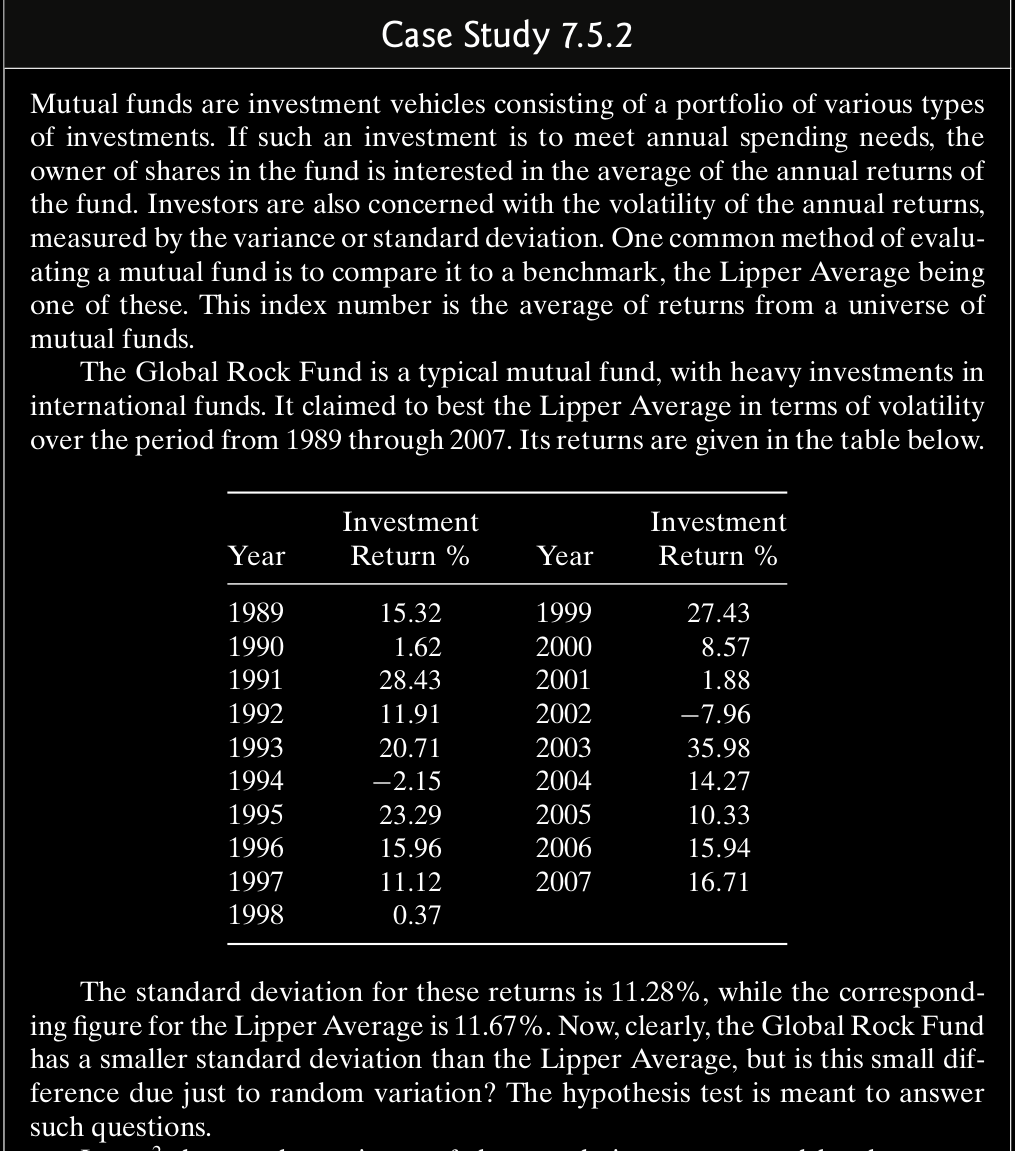
\includegraphics[scale=0.23]{Case_7-5-2-neg.png}
\end{frame}
%-------------- end slide -------------------------------%}}}
%-------------- start slide -------------------------------%{{{ 7.52
\begin{frame}
\centering
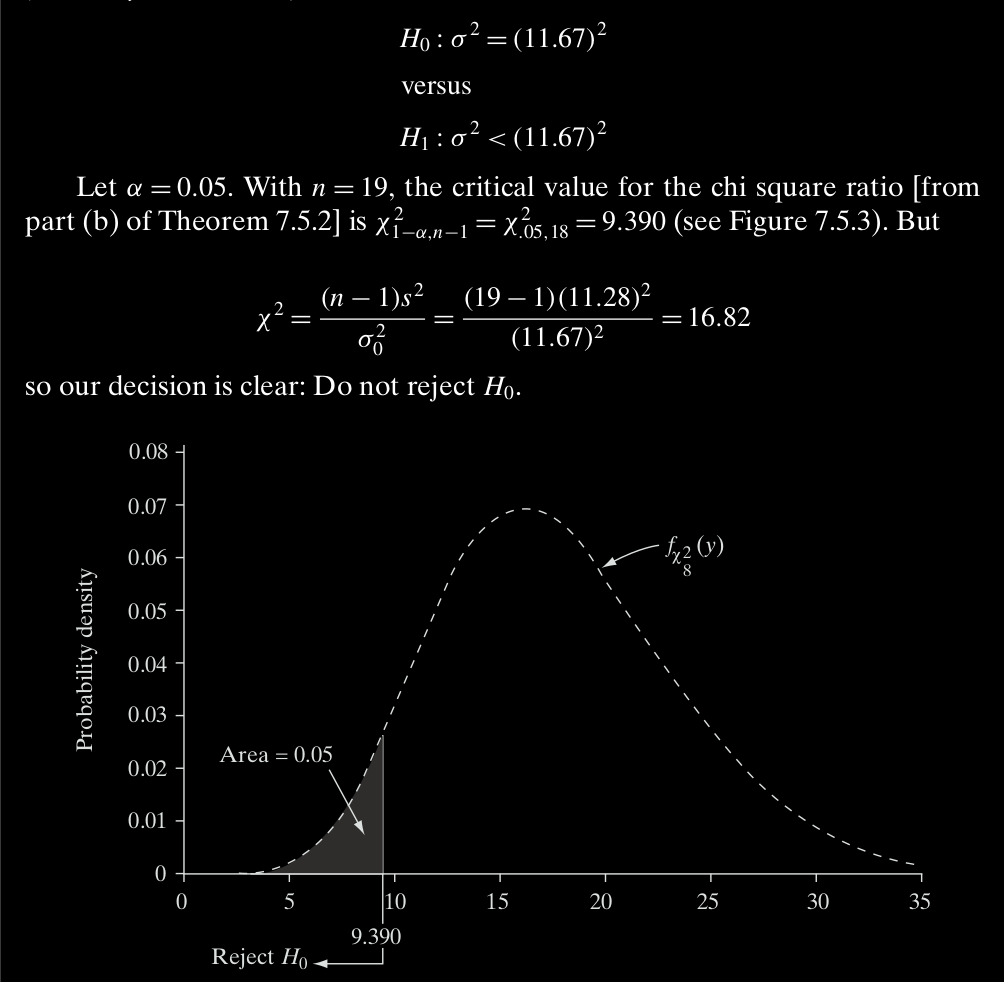
\includegraphics[scale=0.25]{Case_7-5-2-2-neg.png}
\end{frame}
%-------------- end slide -------------------------------%}}}
